\documentclass{thesisclass}


% Based on thesisclass of Timo Rohrberg, 2009
% ----------------------------------------------------------------
% Thesis - Main document
% ----------------------------------------------------------------


%% -------------------------------
%% |  Information for PDF file   |
%% -------------------------------
\hypersetup{
 pdfauthor={Not set},
 pdftitle={Not set},
 pdfsubject={Not set},
 pdfkeywords={Not set}
}


%% ---------------------------------
%% | Information about the thesis  |
%% ---------------------------------

\newcommand{\myname}{Vanessa Wiedmann}
\newcommand{\mytitle}{Systematische Untersuchungen zur Hochspannungskalibration\\ 
											und -stabilisierung am Monitor-Spektrometer}
\newcommand{\myinstitute}{Institut f�r Kernpysik (IK)}

\newcommand{\reviewerone}{}
\newcommand{\reviewertwo}{}
\newcommand{\advisor}{}
\newcommand{\advisortwo}{}

\newcommand{\timestart}{01. April 2011}
\newcommand{\timeend}{01. April 2012}
\newcommand{\submissiontime}{DD. MM. 20XX}


%% ---------------------------------
%% | ToDo Marker - only for draft! |
%% ---------------------------------
% Remove this section for final version!
\setlength{\marginparwidth}{20mm}

\newcommand{\margtodo}
{\marginpar{\textbf{\textcolor{red}{ToDo}}}{}}

\newcommand{\todo}[1]
{{\textbf{\textcolor{red}{(\margtodo{}#1)}}}{}}


%% --------------------------------
%% | Old Marker - only for draft! |
%% --------------------------------
% Remove this section for final version!
\newenvironment{deprecated}
{\begin{color}{gray}}
{\end{color}}


%% --------------------------------
%% | Settings for word separation |
%% --------------------------------
% Help for separation:
% In 



% package the following hints are additionally available:
% "- = Additional separation
% "| = Suppress ligation and possible separation (e.g. Schaf"|fell)
% "~ = Hyphenation without separation (e.g. bergauf und "~ab)
% "= = Hyphenation with separation before and after
% "" = Separation without a hyphenation (e.g. und/""oder)

% Describe separation hints here:
\hyphenation{
% Pro-to-koll-in-stan-zen
% Ma-na-ge-ment  Netz-werk-ele-men-ten
% Netz-werk Netz-werk-re-ser-vie-rung
% Netz-werk-adap-ter Fein-ju-stier-ung
% Da-ten-strom-spe-zi-fi-ka-tion Pa-ket-rumpf
% Kon-troll-in-stanz
}


%% ------------------------
%% |    Including files   |
%% ------------------------
% Only files listed here will be included!
% Userful command for partially translating the document (for bug-fixing e.g.)
%\includeonly{
%titlepage,
%introduction,
%content,
%evaluation,
%conclusion,
%appendix
%}


%%%%%%%%%%%%%%%%%%%%%%%%%%%%%%%%%
%% Here, main documents begins %%
%%%%%%%%%%%%%%%%%%%%%%%%%%%%%%%%%
\begin{document}


\frontmatter
\pagenumbering{roman}
%% titlepage.tex
%%

% coordinates for the bg shape on the titlepage
\newcommand{\diameter}{20}
\newcommand{\xone}{-15}
\newcommand{\xtwo}{160}
\newcommand{\yone}{15}
\newcommand{\ytwo}{-253}

\begin{titlepage}
% bg shape
\begin{tikzpicture}[overlay]
\draw[color=gray]  
 		 (\xone mm, \yone mm)
  -- (\xtwo mm, \yone mm)
 arc (90:0:\diameter pt) 
  -- (\xtwo mm + \diameter pt , \ytwo mm) 
	-- (\xone mm + \diameter pt , \ytwo mm)
 arc (270:180:\diameter pt)
	-- (\xone mm, \yone mm);
\end{tikzpicture}
	\begin{textblock}{10}[0,0](4,2.5)
		
\includegraphics[width=.3\textwidth]{logos/KITLogo_RGB.pdf}
	\end{textblock}
	\changefont{phv}{m}{n}	% helvetica	
	\vspace*{3.5cm}
	\begin{center}
		\Huge{\mytitle}
		\vspace*{2cm}\\
		\Large{
			\iflanguage{english}{Diploma Thesis of}			
												  {Diplomarbeit\\von }
		}\\
		\vspace*{1cm}
		\huge{\myname}\\
		\vspace*{1cm}
		\Large{
			\iflanguage{english}{At the Department of Informatics}			
													{An der Fakult\"at f\"ur Physik}
			\\
			\myinstitute
		}
	\end{center}
	\vspace*{1cm}
\Large{
\begin{center}
\begin{tabular}[ht]{l c l}
  % Gutachter sind die Professoren, die die Arbeit bewerten. 
  \iflanguage{english}{Reviewer}{Erstgutachter}: Prof. Guido Drexlin& \hfill  \\
  \iflanguage{english}{Second reviewer}{Zweitgutachter}: Prof. Michael Feindt& \hfill  \\
  \iflanguage{english}{Advisor}{Betreuender Mitarbeiter}: Dr. Thomas Th�mmler& \hfill  \\
\end{tabular}
\end{center}
}


\vspace{2cm}
\begin{center}
\large{\iflanguage{english}{Duration:}{Bearbeitungszeit}: \timestart \hspace*{0.25cm} -- \hspace*{0.25cm} \timeend}
\end{center}


\begin{textblock}{10}[0,0](4,16.8)
\tiny{ 
	\iflanguage{english}
		{KIT -- University of the State of Baden-Wuerttemberg and National Laboratory of the Helmholtz Association}
		{KIT -- Universit\"at des Landes Baden-W\"urttemberg und nationales Forschungszentrum der Helmholtz-Gesellschaft}
}
\end{textblock}

\begin{textblock}{10}[0,0](14,16.75)
\large{
	\textbf{www.kit.edu} 
}
\end{textblock}

\end{titlepage}

\blankpage


%% -------------------
%% |   Directories   |
%% -------------------
\tableofcontents
\blankpage


%% -----------------
%% |   Main part   |
%% -----------------
\mainmatter
\pagenumbering{arabic}
%% Einleitung.tex
%%

%% ==============================
\chapter{Einleitung}
\label{ch:Einleitung}
%% ==============================



\begin{quotation}
\itshape
I have done something very bad today by proposing a particle that can not be detected. That's something no theorist should ever do. \newline
\normalfont
- Wolfgang Pauli 
\end{quotation} 


Im Jahre 1930 postulierte Wolfgang Pauli das Neutrino, wodurch die bis dahin ungekl�rte Form des kontinuierlichen Spektrums bei Beta-Zerf�llen erkl�rt werden konnte.
Das elektrisch neutrale Neutrino muss eine sehr kleiner Masse haben und war somit mit den damaligen Experimenten nicht Nachweisbar.
Erst 26 Jahre sp�ter gelang es beim Cowan-Reines-Neutrinoexperiment \cite{COWANREINES} Neutrinos nachzuweisen.
Und auch heute noch sind Neutrinos und ihre Eigenschaften fester Bestandteil vieler Experimente und von gro�em Interesse f�r die Physik.
Vor kurzem Schokierte OPERA \cite{OPERA} die Physik-Welt mit dem Ergebniss, dass Neutrinos 60ns schneller als Licht w�ren. 
RENO ver�ffentlicht vermutlich im Juni 2012 ihre Ergebnisse f�r den Mischungswinkel $\theta_{13}$ und KATRIN m�chte im Jahre 2015 eine neue Obergrenze f�r die Neutrinomasse gemessen haben. Okay, der letzte Satz ist schei�e. Aber ich versuche mal im Flow zu bleiben.

 
test \cite{RGr}







%\cite{OPERA}
lalala
%% Neutrinos.tex
%%

%% ==============================
\chapter{Neutrinos}
\label{ch:Neutrinos}
%% ==============================
Hier kommen tolle dinge �ber neutrinos. Wohhooo

\section{Das Standardmodel}
\section{Neutrinoquellen}
\subsection{Solare Neutrinos}
\subsection{Atmosph�rische Neutrinos}
\subsection{Reaktor-Neutrinos}
\subsection{Beschleuniger-Neutrinos}
\section{Neutrino-Oszillation}
Neutrino-Oszillation ist der erste Beweis f�r Physik jenseits des Standardmodells.


\section{Massenbestimmung}
\subsection{TOF}
\subsection{Neutrinoloser Doppelbeta-Zerfall}
\subsection{Beta-Spektrum}

%%KATRIN-Experiment.tex
%%

%% ==============
\chapter{Das KATRIN-Experiment}
\label{ch:Das KATRIN-Experiment}
%% ==============

Was macht Katrin, Neutrinomasse, unerreichte Senistivit�t usw.

\begin{figure}[ht]%
\centering
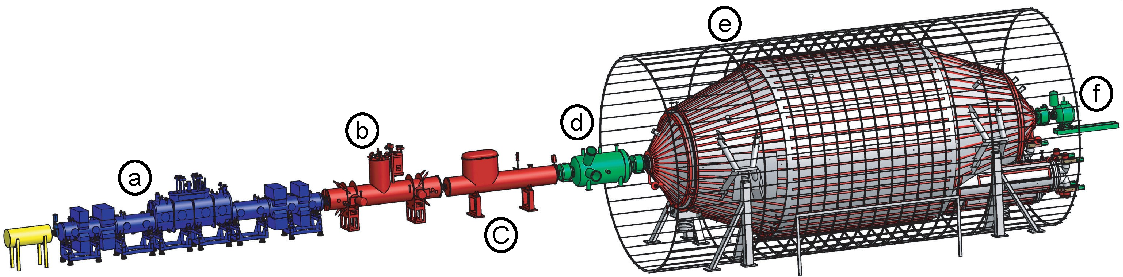
\includegraphics[width=\columnwidth]{Bilder/KATRIN/KATRIN_uebersicht.pdf}%
\caption[Aufbau des KATRIN-Experiments]{Der Aufbau des KATRIN-Experiments: Die fensterlose Quelle in blau (a), mit der Rear-Section in gelb, die differentielle (b) und kryogene (c) Pumpstrecke, das Vorspektrometer (d) sowie das Hauptspektrometer (e) mit seinen Luftspulensystemen und der Elektronendetektor (f) \cite{DTReich}}%
\label{fig:KATRIN_uebersicht}%
\end{figure}


%% ===========================

\section{Tritiumspektrum}
\section{MAC-E-Filter}
\section{Transmissionsfunktion}
\section{Aufbau von KATRIN}
\subsection{Fensterlose gasf�rmige Tritiumquelle}
\subsection{Spektrometer}
\subsection{Detektor}
%% ===========================

\section{Hochspannungslayout}

\dots

%% Das Monitorspektrometer.tex
%%

%% ==============
\chapter{Das Monitorspektrometer}
\label{ch:Monitorspektrometer}
%% ==============

Das Monitorspektrometer stammt von dem Mainzer Neutrinomassenexperiment


%% ===========================
\section{Quelle}
\label{ch:Monitorspektrometer:sec:Quelle}
%% ===========================

%% ===========================
\section{Detektor}
\label{ch:Monitorspektrometer:sec:Detektor}
%% ===========================


%% ===========================
\section{Hochspannungslayout}
\label{ch:Monitorspektrometer:sec:Hochspannungslayout}
%% ===========================


%% ===========================
\section{Nachregelung}

%% ===========================


%%Messungen.tex
%%

%% ==============
\chapter{Messungen am Monitorspektrometer}
\label{ch:Messungen}
%% ==============

So wird normalerweise gemessen


\section{Implementierung der St�rung in die Transmissionsfunktion}
\label{ch:Messungen:sec:Transmissionsfunktion}

%% ===========================
\section{St�rungen an der Quelle}
\label{ch:Messungen:sec:St�rungen}
%% ===========================


%% ===========================
\subsection{Auswertung}
\label{ch:Messungen:sec:AuswertungQuelle}
%% ===========================

%% ===========================
\subsection{Ergebnisse}
\label{ch:Messungen:sec:ErgebnisseQuelle}
%% ===========================

\section{St�rungen des Tankpotentials}
\label{ch:Messungen:sec:Tank}

%% ===========================
\subsection{Auswertung}
\label{ch:Messungen:sec:AuswertungTank}
%% ===========================

%% ===========================
\subsection{Ergebnisse}
\label{ch:Messungen:sec:ErgebnisseTank}
%% ===========================
\dots

%% Zusammenfassung und Ausblick.tex
%%

%% ==================
\chapter{Zusammenfassung und Ausblick}
\label{ch:Zusammenfassung}
%% ==================

\dots


%% --------------------
%% |   
%bibliography   |
%% --------------------
\cleardoublepage
\phantomsection
\addcontentsline{toc}{chapter}{\bibname}

\iflanguage{english}
{\bibliographystyle{IEEEtranSA}}	% english style
{\bibliographystyle{babalpha-fl}}	% german style
												  
% Use IEEEtran for numeric references
%\bibliographystyle{IEEEtranSA})

\bibliography{bibliography}



%% ----------------
%% |   Appendix   |
%% ----------------
\cleardoublepage

%% appendix.tex
%%

%% ==============================
%\chapter{Appendix}
%\label{ch:Appendix}
%% ==============================

\appendix

\iflanguage{english}
{\addchap{Appendix}}	% english style
{\addchap{Anhang}}	% german style


\listoffigures


\section{First Appendix Section}
		\label{Anhang-Implementierung}
		
\setcounter{figure}{0}
		
\begin{figure} [ht]
  \centering
   ein Bild
  \caption{A figure}
  \label{fig:BPMNBeispiela}
\end{figure}


\dots






\end{document}
